\documentclass[10pt]{scrartcl}
\usepackage[mdthm,colorsec,noauthor,noasy]{evan}
\usepackage{handout}
\title{CS 61A --- Week 1}
\subtitle{Expressions, names, functions, environment diagrams, print and None (Lectures 1--2, Composing Programs 1.1--1.3)}
\author{}\date{}\ihead{}
\begin{document}
\maketitle

\section{This week}

\subsection{Expressions and how Python evaluates them}

\begin{qbox}
  A program is text. What exactly does Python do, step by step, to turn the text \cd{mul(add(4, mul(4, 6)), add(3, 5))} into the number \cd{224}? Every ``What Would Python Display'' exam question is this question.
\end{qbox}

\begin{itemize}
  \ii An \vocab{expression} describes a computation and \vocab{evaluates to a value}. \cd{2026}, \cd{'hello'}, \cd{2 + 3}, \cd{max(1, 2)} are expressions.
  \ii Values have types. This week: numbers (\cd{6}, \cd{2.5}), strings (\cd{'are you human'}), functions (\cd{pow}), and the special value \cd{None}.
  \ii A \vocab{call expression} has the form \emph{operator}\cd{(}\emph{operand}\cd{,} \dots\cd{)}. In \cd{max(1 + 1, 3)} the operator is \cd{max} and the operands are \cd{1 + 1} and \cd{3}. The operator and the operands are themselves expressions.
  \ii Every arithmetic expression can be written as a call: \cd{2 + 3} is \cd{add(2, 3)}, \cd{2 * 3} is \cd{mul(2, 3)} (after \cd{from operator import add, mul}).
\end{itemize}

\method{Evaluation procedure for a call expression.}
\begin{steps}
  \ii Evaluate the operator. Its value must be a function.
  \ii Evaluate each operand, from left to right. Their values are the \vocab{arguments}.
  \ii Apply the function to the arguments. The result is the value of the call expression.
\end{steps}
\begin{ideabox}
The procedure refers to itself: step 2 says ``evaluate each operand'', and an operand may be another call expression, which is evaluated by the same three steps. So a nested expression is evaluated from the inside out, and among operands at the same level, from left to right.

The order matters as soon as evaluating an operand \emph{does} something visible, such as printing. On exams, the order of the displayed lines is decided by this procedure and by nothing else.
\end{ideabox}
\begin{fig}
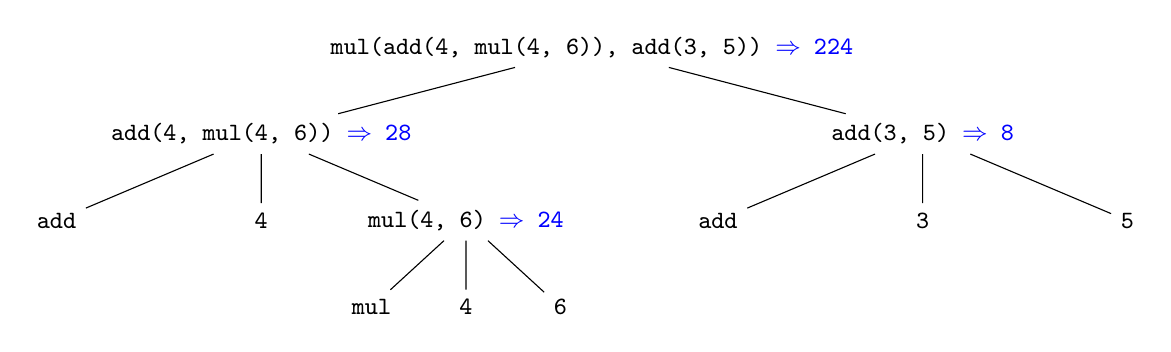
\begin{tikzpicture}[level distance=11mm,
  level 1/.style={sibling distance=84mm},level 2/.style={sibling distance=26mm},level 3/.style={sibling distance=12mm},
  every node/.style={font=\ttfamily\small},val/.style={draw=blue!60,rounded corners=2pt,inner sep=2pt,font=\ttfamily\small\color{blue}}]
  \node {mul(add(4, mul(4, 6)), add(3, 5)) \textrm{\color{blue}$\Rightarrow$} \color{blue}224}
    child {node {add(4, mul(4, 6)) \textrm{\color{blue}$\Rightarrow$} \color{blue}28}
      child {node {add}}
      child {node {4}}
      child {node {mul(4, 6) \textrm{\color{blue}$\Rightarrow$} \color{blue}24}
        child {node {mul}} child {node {4}} child {node {6}}}}
    child {node {add(3, 5) \textrm{\color{blue}$\Rightarrow$} \color{blue}8}
      child {node {add}} child {node {3}} child {node {5}}};
\end{tikzpicture}
\figcap{Expression tree. Each call expression is evaluated after its operator and operands. Order in which the calls finish: \cd{mul(4, 6)}, then \cd{add(4, 24)}, then \cd{add(3, 5)}, then \cd{mul(28, 8)}.}
\end{fig}

\textbf{Arithmetic operators you will use constantly.}
\begin{itemize}
  \ii \cd{/} is true division and always gives a float: \cd{6 / 3} is \cd{2.0}. \cd{//} is floor division: \cd{7 // 2} is \cd{3}. \cd{\%} is remainder: \cd{7 \% 2} is \cd{1}. \cd{**} is power: \cd{2 ** 10} is \cd{1024}.
  \ii For a positive integer \cd{n}: \cd{n \% 10} is its last digit and \cd{n // 10} is \cd{n} with the last digit removed. (\cd{2026 \% 10} is \cd{6}; \cd{2026 // 10} is \cd{202}.)
  \ii \cd{n \% d == 0} tests whether \cd{d} divides \cd{n} evenly.
\end{itemize}

\subsection{Names and assignment}

\begin{qbox}
  After \cd{x = 2}, then \cd{y = x + 1}, then \cd{x = 5}: what is \cd{y}?
\end{qbox}
\method{Execution rule for an assignment statement} \cd{name = expression}:
\begin{steps}
  \ii Evaluate the expression on the right.
  \ii Bind the name on the left to that \emph{value} in the current frame (replacing any earlier binding of the name).
\end{steps}
\begin{ideabox}
A name is bound to a value, never to another name or to an expression. When \cd{y = x + 1} runs, Python computes \cd{3} and binds \cd{y} to \cd{3}. Nothing remembers that the \cd{3} came from \cd{x}. So changing \cd{x} later cannot change \cd{y}.
\end{ideabox}
\begin{py}
>>> x = 2
>>> y = x + 1
>>> x = 5
>>> y
3
\end{py}
\begin{itemize}
  \ii \textbf{Functions are values, so names can be bound to them.} From lecture:
\end{itemize}
\begin{py}
>>> max = pow        # the name max is now bound to the function pow
>>> max(2, 5 + 5)    # operator evaluates to pow; operands to 2 and 10
1024
\end{py}
\begin{itemize}
  \ii The name \cd{pow} is unchanged, and the function that used to be called \cd{max} is no longer reachable by that name.
  \ii \textbf{Multiple assignment}: all expressions on the right are evaluated \emph{before} any name is bound. So \cd{x, y = y, x} swaps the two values.
  \ii \cd{from operator import add, mul} and \cd{from math import sqrt, pi} bind names to values from a library.
\end{itemize}

\subsection{Defining and calling functions}

\begin{py}
def g(y):
    x = 2 * y
    return x + 1
\end{py}
\begin{itemize}
  \ii A \cd{def} statement creates a function and binds its name (\cd{g}) to it in the current frame. \textbf{The body is not executed when the function is defined.} It is executed each time the function is called.
  \ii \cd{y} is the \vocab{formal parameter}. The first line \cd{def g(y):} is the \vocab{signature}.
  \ii A \cd{return} statement evaluates its expression, ends the call, and makes that value the value of the call expression.
\end{itemize}

\method{Procedure for calling a user-defined function.}
\begin{steps}
  \ii Add a new \vocab{local frame}.
  \ii Bind the function's formal parameters to the arguments in that frame.
  \ii Execute the body of the function in the environment that starts with that frame.
\end{steps}

\subsection{Frames, environments, and environment diagrams}

\begin{qbox}
  The function \cd{g} above uses the name \cd{x}, and the program that calls it may also use \cd{x}. Which \cd{x} is meant where, and can one overwrite the other?
\end{qbox}
\begin{itemize}
  \ii A \vocab{frame} holds bindings of names to values. A name appears at most once in a frame.
  \ii The \vocab{global frame} holds the names defined at the top level (and gives access to the built-in names such as \cd{max}, \cd{pow}).
  \ii An \vocab{environment} is a sequence of frames: a local frame followed by the global frame, or the global frame alone. (From Week 2 on, the sequence can be longer.)
  \ii \textbf{Lookup rule}: a name evaluates to the value bound to it in the \emph{earliest} frame of the current environment in which the name is found. Local frame first, then global.
  \ii An assignment inside a function body binds the name in the \emph{local} frame. It does not change any other frame.
\end{itemize}
\begin{ideabox}
Why organise names this way? The person who writes \cd{g} should be free to choose the names \cd{x} and \cd{y} without knowing which names the rest of the program uses. Local frames give that: every call gets a fresh frame, the body looks there first, and assignments in the body stay there. When the call returns, the frame is no longer used.

An environment diagram is the bookkeeping for these rules. Drawing one is slow but mechanical, and it removes all guessing from questions about what a name refers to.
\end{ideabox}
\Needspace{24\baselineskip}
\textbf{Worked example (from lecture).} Trace this program:
\begin{py}
def g(y):
    x = 2 * y
    return x + 1

x = 2
print(g(3 * x) + 3)
print(x)
\end{py}
\begin{steps}
  \ii \cd{def}: bind \cd{g} in the global frame to a new function.
  \ii \cd{x = 2}: bind \cd{x} to \cd{2} in the global frame.
  \ii Evaluate \cd{g(3 * x) + 3}. First the call \cd{g(3 * x)}: the operator \cd{g} is the function; the operand \cd{3 * x} is evaluated in the global frame and gives \cd{6}.
  \ii Call \cd{g} with argument \cd{6}: new frame \cd{f1}; bind \cd{y} to \cd{6}.
  \ii Body, line 1: \cd{2 * y} looks up \cd{y} in \cd{f1}: \cd{12}. Bind \cd{x} to \cd{12} \emph{in \cd{f1}}. The global \cd{x} is still \cd{2}.
  \ii Body, line 2: \cd{x + 1} looks up \cd{x}; it is found in \cd{f1} first: \cd{13}. Return \cd{13}.
  \ii Back in the global frame: \cd{13 + 3} is \cd{16}; \cd{print} displays \cd{16}.
  \ii \cd{print(x)}: \cd{x} is looked up in the global frame: displays \cd{2}.
\end{steps}
\begin{fig}
\begin{tikzpicture}[>=Stealth,font=\ttfamily\small]
  \draw[thick] (0,0) rectangle (4.6,1.5); \node[anchor=west,font=\small\bfseries] at (0,1.75) {Global frame};
  \node[anchor=east] at (2.0,1.05) {g}; \draw (2.1,0.8) rectangle (4.4,1.3);
  \node[anchor=east] at (2.0,0.4) {x}; \draw (2.1,0.15) rectangle (4.4,0.65); \node at (3.25,0.4) {2};
  \fill (3.25,1.05) circle (1.5pt); \draw[->] (3.25,1.05) -- (6.2,1.05);
  \node[anchor=west] at (6.3,1.05) {func g(y) [parent=Global]};
  \draw[thick] (0,-3.1) rectangle (4.6,-0.9); \node[anchor=west,font=\small\bfseries] at (0,-0.65) {f1: g [parent=Global]};
  \node[anchor=east] at (2.0,-1.3) {y}; \draw (2.1,-1.55) rectangle (4.4,-1.05); \node at (3.25,-1.3) {6};
  \node[anchor=east] at (2.0,-1.95) {x}; \draw (2.1,-2.2) rectangle (4.4,-1.7); \node at (3.25,-1.95) {12};
  \node[anchor=east,font=\small] at (2.0,-2.6) {\rmfamily Return value}; \draw (2.1,-2.85) rectangle (4.4,-2.35); \node at (3.25,-2.6) {13};
  \node[anchor=west,text width=6.6cm,font=\rmfamily\small] at (6.3,-1.9) {Two different bindings of \cd{x}. Inside the call, lookup finds \cd{x} in \cd{f1} first (12). After the call, the current environment is the global frame alone, where \cd{x} is 2.};
\end{tikzpicture}
\figcap{Environment diagram at the moment \cd{g} returns. The frame label records the function's name and its parent.}
\end{fig}

\method{How to draw an environment diagram.}
\begin{steps}
  \ii Start with the global frame. Execute statements one at a time, in order.
  \ii \cd{def}: write the function value \cd{func name(params) [parent=\emph{current frame}]} and bind the name to it.
  \ii Assignment: evaluate the right side completely, then write or overwrite the binding in the current frame.
  \ii Call to a user-defined function: evaluate operator and operands first (in the current environment). Then open a new frame labelled \cd{f1}, \cd{f2}, \dots with the function's \emph{original} name (the name in its \cd{def}) and its parent; bind the parameters; run the body.
  \ii \cd{return}: write the return value in the frame. A function whose body finishes without \cd{return} returns \cd{None}.
  \ii Calls to built-in functions (\cd{print}, \cd{max}, \cd{add}) do not get a frame in the diagram.
\end{steps}

\textbf{Name conflicts (from lecture).}
\begin{py}
from operator import mul
def square(square):
    return mul(square, square)
square(3)
\end{py}
\begin{itemize}
  \ii In the global frame, \cd{square} is the function. The call \cd{square(3)} opens \cd{f1} and binds the \emph{parameter} \cd{square} to \cd{3} there.
  \ii In the body, \cd{square} is looked up in \cd{f1} first and is \cd{3}; \cd{mul} is not in \cd{f1}, so it is found in the global frame. The result is \cd{9}.
  \ii It works, but inside the body the function can no longer be reached by the name \cd{square}. Do not reuse names like this.
\end{itemize}

\subsection{print, return, and None}

\begin{qbox}
  \cd{print(x)} and \cd{return x} both seem to ``give back'' \cd{x}. What is the difference, and why does \cd{None} show up in exam answers?
\end{qbox}
\begin{itemize}
  \ii \cd{return} hands a value to the caller. Nothing is displayed.
  \ii \cd{print} \emph{displays} its arguments (separated by spaces) and \emph{returns} \cd{None}.
  \ii \cd{None} is a value that represents nothing. A function without a \cd{return} statement returns \cd{None}.
  \ii A \vocab{pure function} only returns a value (\cd{abs}, \cd{pow}, \cd{add}). A \vocab{non-pure function} also has a side effect, such as displaying output (\cd{print}).
  \ii \textbf{The interactive interpreter} (\cd{>>>}) displays the value of each expression you type, \emph{unless that value is \cd{None}}. A file run with \cd{python3 file.py} displays only what is printed.
  \ii In the interpreter a string value is displayed with quotes (\cd{'hi'}); \cd{print('hi')} displays \cd{hi} without quotes.
\end{itemize}
\begin{py}
>>> -2            # value displayed
-2
>>> print(-2)     # displayed by print; the value None is not displayed
-2
>>> None          # nothing displayed
>>> print(None)   # print displays the word None
None
>>> print(print(1), print(2))
1
2
None None
\end{py}
\begin{ideabox}
The last example is the model for every nested-print question. Apply the evaluation procedure to the outer call: its operands \cd{print(1)} and \cd{print(2)} must be evaluated first, left to right. Evaluating \cd{print(1)} displays \cd{1} and has value \cd{None}; evaluating \cd{print(2)} displays \cd{2} and has value \cd{None}. Only then is the outer \cd{print} applied, to the arguments \cd{None} and \cd{None}, so it displays \cd{None None}. The outer call's own value is \cd{None}, which the interpreter does not display.
\end{ideabox}
\textbf{The lecture's \cd{noisy} example.}
\begin{py}
def noisy(x):
    print('NOISY', x)
    return x + 1

>>> noisy(noisy(2) + noisy(3))
NOISY 2
NOISY 3
NOISY 7
8
\end{py}
\begin{steps}
  \ii The operand \cd{noisy(2) + noisy(3)} is evaluated first. \cd{noisy(2)} displays \cd{NOISY 2} and returns \cd{3}.
  \ii \cd{noisy(3)} displays \cd{NOISY 3} and returns \cd{4}. The operand's value is \cd{7}.
  \ii The outer call \cd{noisy(7)} displays \cd{NOISY 7} and returns \cd{8}.
  \ii The interpreter displays the value \cd{8}.
\end{steps}
If \cd{noisy} used \cd{print(x + 1)} instead of \cd{return x + 1}, then \cd{noisy(2)} would return \cd{None}, and \cd{None + None} is an error.

\textbf{Search, the lecture's closing example.} Discussion 0 asked for the shortest expression built from \cd{f(x) = x + 1}, \cd{g(x) = 2 * x - 1}, \cd{h(x, y)} (concatenate digits) and the number \cd{5} that evaluates to \cd{2026}. The lecture's program tries every expression with 3 calls, then 4 calls, and so on, and finds \cd{f(g(h(f(g(5)),g(f(f(5))))))} with 8 calls. The point for the course: a program can examine many alternatives by repeating simple operations. The code uses classes, generators and recursion, which come later.

\begin{shortcuts}
  \ii \textbf{What Would Python Display}: work one line at a time. For each line write, in order, (1) everything displayed while operands are evaluated, left to right and inside out, then (2) what the outermost call displays, then (3) the line's value if you are at \cd{>>>} and it is not \cd{None}.
  \ii \textbf{Label every call with its return value} as you go. For \cd{print} the label is always \cd{None}.
  \ii \textbf{Last digit / the rest}: \cd{n \% 10} and \cd{n // 10}.
  \ii \textbf{Environment diagrams}: an assignment never changes another frame; the frame label uses the name from the \cd{def} line, not the name used in the call.
  \ii \textbf{Is the body run now?} Not at \cd{def}; only at a call. A name that does not exist inside a body causes an error only when that line is executed.
  \ii \textbf{Operands before the call}: an operand is evaluated in the frame where the call expression is written, not in the new frame.
\end{shortcuts}
\begin{trapbox}
  \ii \cd{print} returns \cd{None}. \cd{x = print(5)} displays \cd{5} and binds \cd{x} to \cd{None}.
  \ii \cd{6 / 3} is \cd{2.0}, not \cd{2}.
  \ii \cd{y = x + 1} does not link \cd{y} to \cd{x}.
  \ii Rebinding a built-in name (\cd{max = pow}) is legal and silently changes what later calls do.
  \ii Forgetting \cd{return}: the function returns \cd{None}, and the error appears later, where the result is used.
  \ii In the interpreter a string value shows quotes; printed, it does not.
\end{trapbox}

\section{Problem set}
These are original problems of the kind asked in lab and on Midterm 1. (The course's own homework, lab and project questions are for you to do without AI help; they are not reproduced or solved here.) Past-exam questions on these topics also use \cd{lambda}, \cd{and}/\cd{or} and \cd{while}, so they appear in the Week 2 and Week 3 handouts. The programming exercises are in \cd{exercises/}.

\begin{prob}\textbf{P1 (evaluation order).}\ Draw the expression tree and give the value: \cd{sub(pow(2, add(1, 2)), mul(2, add(1, 1)))}. In which order do the five calls finish?
\end{prob}
\begin{prob}\textbf{P2 (assignment).}\ What is displayed?
\begin{py}
>>> a = 3
>>> b = a * 2
>>> a = b - 1
>>> a, b = b, a + b
>>> a
>>> b
\end{py}
\end{prob}
\begin{prob}\textbf{P3 (names bound to functions).}\ What is displayed?
\begin{py}
>>> f = min
>>> min = max
>>> max = f
>>> min(1, 2) + max(3, 4)
\end{py}
\end{prob}
\begin{prob}\textbf{P4 (print and None).}\ What is displayed? Write \cd{ERROR} if an error occurs.
\begin{py}
>>> x = print(1, 2)
>>> x
>>> print(x)
>>> print(print(3), 4)
>>> print(7) + 1
\end{py}
\end{prob}
\begin{prob}\textbf{P5 (return versus print).}\ What is displayed?
\begin{py}
def loud(x):
    print('got', x)
    return 2 * x

def quiet(x):
    print(2 * x)

>>> loud(loud(1))
>>> quiet(quiet(1))
\end{py}
\end{prob}
\begin{prob}\textbf{P6 (environment diagram).}\ Draw the environment diagram and give what is displayed.
\begin{py}
def f(x, y):
    x = x + y
    y = x * 2
    return y - x

x = 3
y = f(x, x + 1)
print(x, y)
\end{py}
\end{prob}
\begin{prob}\textbf{P7 (parameters shadow globals).}\ What is displayed?
\begin{py}
from operator import add
def add(add, mul):
    return mul

x = add(1, 2)
print(x)
print(add(add, x))
\end{py}
\end{prob}
\begin{prob}\textbf{P8 (body runs only when called).}\ Which line, if any, causes an error, and when?
\begin{py}
def h(n):
    return n + undefined_name

z = 10
print(z)
print(h(z))
\end{py}
\end{prob}

\end{document}
